\documentclass[letterpaper, 10pt, conference]{ieeeconf}
\IEEEoverridecommandlockouts
\overrideIEEEmargins

\usepackage[utf8]{inputenc}
\usepackage[T1]{fontenc}
\usepackage{graphicx}
\usepackage{amsmath,amssymb}
\usepackage{booktabs}
\usepackage{multirow}
\usepackage{subfig}
\usepackage{hyperref}

\title{\LARGE \bf Optimization and Uncertainty in Learning on Forest Cover Type}

\author{Tanxin Liu\\
  Georgia Institute of Technology\\
  \texttt{tliu626@gatech.edu}}

\begin{document}
\maketitle
\thispagestyle{empty}
\pagestyle{empty}

%-------------------------------------------------------------------------------
\begin{abstract}
Using the PyTorch neural network finalized in our Supervised Learning (SL)
Report as a fixed backbone, we study how optimization and regularization choices
shape training dynamics, generalization, stability, and compute cost on the
seven-class, imbalanced Forest Cover Type task. The backbone is a single
$150$-unit ReLU multilayer perceptron trained with class-weighted cross-entropy;
the SL SGD-only network is the reference baseline (test Macro-F1~$0.625$,
balanced accuracy~$0.767$). Three interventions are compared under fixed,
reported budgets: randomized optimization(RO) (Randomized Hill Climbing (RHC), Simulated Annealing (SA), Genetic Algorithm (GA)) on the final classifier
layer ($1{,}057$ parameters); Adam-family optimizer ablations; and a
regularization study with standard Adam. We find a consistent \emph{dissociation}
between validation loss and classification quality. Genetic search drove
validation cross-entropy well below the baseline ($0.544$ vs.\ $0.686$) yet
\emph{reduced} Macro-F1 to $0.578$; the RMSProp-like Adam variant
($\beta_1{=}0$) gave the best test Macro-F1 ($0.649$) and balanced accuracy
($0.773$); momentum and Nesterov overfit most (largest train--validation gaps);
and L2 weight decay halved the generalization gap and gave the highest balanced
accuracy while slightly lowering Macro-F1. Adding final-layer RO on top of the
best Adam-plus-regularization recipe did not help. We accept our hypotheses:
adaptive scaling reaches a validation-loss threshold fastest, but speed and
lower loss do not transfer to Macro-F1; regularization primarily controls the
generalization gap and minority-class recall; and final-layer RO is not worth
its function-evaluation cost.
\end{abstract}

%-------------------------------------------------------------------------------
\section{Introduction}
\label{sec:intro}

Machine-learning projects rarely fail because a model cannot learn; they fail
because the wrong training levers are pulled, in the wrong order, and coincidence
is mistaken for causation. Building directly on the SL Report, we
reuse the same Forest Cover Type sample, target, split strategy, preprocessing,
and PyTorch backbone, and ask a different question: not \emph{which} model wins,
but \emph{how} optimization and regulation choices affect validation loss, Macro-F1,
balanced accuracy, class-level behavior, seed stability, and compute cost under
controlled budgets~\cite{blackard1999}.

Our SL PyTorch SGD-only network is the baseline reference point for every
comparison; it is not necessarily the strongest SL model (SVM-RBF was), but the
OL study is about the training process of this one backbone. We interrogate
three forces that shape modern training: (i) randomized optimization (RO) applied
to the final classifier layer under a strict parameter cap; (ii) Adam-family
optimizer ablations that separate momentum, Nesterov acceleration, adaptive
scaling, bias correction, and decoupled weight decay~\cite{kingma2015,loshchilov2019};
and (iii) regularization under a fixed optimizer~\cite{srivastava2014,muller2019}.
Uncertainty is treated operationally through seed sensitivity, trajectory
variance, and minority-class variability under fixed compute.

%-------------------------------------------------------------------------------
\section{Data, Baseline, and Experimental Setup}
\label{sec:setup}

\subsection{Dataset, sample, and SL continuity}
The target is \texttt{Cover\_Type} (classes 1--7), a multiclass classification
problem. We reuse the \emph{identical} stratified $20{,}000$-instance sample from
the SL Report (seed\,=\,42), preserving the $103{:}1$ majority-to-minority
imbalance: Lodgepole Pine (C2) is $48.8\%$ of instances while Cottonwood/Willow
(C4) is only $0.47\%$. A single stratified $80/20$ split (seed\,=\,42) reproduces
the SL held-out test set exactly (Table~\ref{tab:setup}); C4 retains only $19$
test instances, so its per-class estimates are high-variance. Preprocessing is
leakage-safe: a \texttt{StandardScaler} is fit on the training continuous columns
only, then applied to validation and test. Labels $1..7$ are mapped to $0..6$.

\begin{table}[t]
\caption{Experimental setup and per-split class counts (identical sample/test
  set to the SL Report). Train:val:test $=12.8$k$:$3.2k$:$4k.}
\label{tab:setup}
\centering\small
\begin{tabular}{@{}lrrrrrrr@{}}
\toprule
Split & C1 & C2 & C3 & C4 & C5 & C6 & C7 \\
\midrule
Train ($12{,}800$) & 4667 & 6241 & 788 & 60 & 210 & 382 & 452 \\
Val   ($3{,}200$)  & 1167 & 1560 & 197 & 15 & 52  & 96  & 113 \\
Test  ($4{,}000$)  & 1458 & 1951 & 246 & 19 & 65  & 120 & 141 \\
\bottomrule
\end{tabular}
\end{table}

\subsection{Backbone and disclosed deviations}
The OL backbone is the finalized SL PyTorch network: a single hidden layer of
$150$ ReLU units ($54{\to}150{\to}7$; $9{,}307$ parameters) trained with
\emph{balanced class-weighted} cross-entropy (C4 receives $\approx30\times$ the
weight of the majority class). The topology is held fixed across all parts; only
Part~3 alters regularization internals. Three deviations from SL are disclosed
for experimental control, so comparisons to the SL number are marked
\emph{approximate}: (a) we carve an explicit training-only validation set ($20\%$
of the train pool) to provide a deterministic RO objective and a threshold for
speed-to-target, whereas SL used a $10\%$ internal split for early stopping; (b)
gradient-based parts use a \emph{fixed} $100$-epoch budget (no early stopping
outside the Part~3 early-stopping condition) so every optimizer receives
identical compute; and (c) the SGD baseline uses no weight decay (SL used
$10^{-4}$). Under these settings the OL baseline reproduces the SL PyTorch
network closely (Macro-F1 $0.625$ vs.\ SL $0.638$; balanced accuracy $0.767$
vs.\ $0.749$; accuracy $0.715$ vs.\ $0.746$).

\subsection{Metrics, compute accounting, and protocol}
We report validation loss, test accuracy, Macro-F1, balanced accuracy, a
confusion matrix, and per-class precision/recall/F1. Macro-F1 and balanced
accuracy are primary because accuracy hides minority-class failure on this
imbalanced target~\cite{sokolova2009,he2009}. Compute is accounted explicitly:
one minibatch backward pass counts as one \emph{gradient evaluation}
(batch\,=\,128, so $100$ batches/epoch, $10{,}000$ per run); one validation
objective call counts as one \emph{function evaluation} for RO; wall-clock is
recorded for every run. GA is compared strictly by function evaluations, not
generations---its $3{,}000$-evaluation budget corresponds to only
$\approx\!100$ generations of population $30$, so a per-generation view would
badly understate its cost. Budgets and the speed-to-target threshold are fixed
in advance (Table~\ref{tab:budget}); runs that do not reach $\ell$ within budget
are marked ``--'' in Table~\ref{tab:part2} and excluded from speed comparisons
(this affected only some momentum/Nesterov seeds). All main claims use three
seeds $\{0,1,2\}$; divergent runs are reported, not deleted. The held-out test
set is touched only at final evaluation. Experiments ran on a single USC CARC
Discovery node (Rocky Linux~8, CPU-only, $8$ cores, PyTorch limited to $4$
threads); software: Python~3.11.9, PyTorch~2.6.0, scikit-learn~1.9, NumPy~2.4,
Pandas~3.0.

\begin{table}[t]
\caption{Fixed compute budgets and the speed-to-target threshold. One backward
  pass = one gradient evaluation; one full-validation objective call = one
  function evaluation.}
\label{tab:budget}
\centering\small
\begin{tabular}{@{}ll@{}}
\toprule
Quantity & Value \\
\midrule
Gradient budget (Parts 0/2/3) & $100$ epochs $=10{,}000$ grad evals \\
RO function-eval budget (Part 1) & $3{,}000$ evals ($\approx100$ GA gens) \\
Part-4 RO budget & $300$ evals ($10\%$ of Part 1) \\
Batch size & $128$ (fixed, matches SL) \\
Speed-to-target $\ell$ & $0.70$ val loss (baseline settles $\approx0.69$) \\
Seeds & $\{0,1,2\}$ \\
\bottomrule
\end{tabular}
\end{table}

\subsection{Hypotheses}
\label{sec:hyp}
Grounded in optimization theory, we fix three hypotheses \emph{before}
experiments. \textbf{H1 (optimization vs.\ generalization).} Adam-family methods
reach a fixed validation-loss threshold with fewer gradient evaluations than SGD
because adaptive second-moment scaling reduces sensitivity to feature and
gradient scale~\cite{kingma2015}; however this speed advantage will \emph{not}
guarantee higher Macro-F1, because errors concentrate in minority cover types
whose decisions loss reductions need not change. \textbf{H2 (regularization).}
Explicit regularization will affect the train--validation gap and minority-class
recall more than optimizer choice, because it changes the full training process
rather than only the update rule~\cite{srivastava2014}. \textbf{H3 (RO cost).}
Final-layer RO will yield small or negative Macro-F1 gains relative to its
function-evaluation cost, since the $1{,}057$-dimensional last-layer objective is
optimized after the representation is frozen and validation-loss gains need not
move hard predictions. We revisit all three in Section~\ref{sec:discussion}.

%-------------------------------------------------------------------------------
\section{Part 1: Randomized Optimization on the Final Layers}
\label{sec:part1}

\subsection{Scope, deterministic objective, and accounting}
The assignment permits RO over the final $1$--$3$ trainable layers under a
$50{,}000$-parameter cap, with the exact trainable count reported. The fixed SL
backbone has only \emph{two} weight-bearing layers ($54{\to}150$ and
$150{\to}7$), so the admissible scope is $1$ or $2$ such layers; unfreezing both
would leave nothing frozen and amount to whole-network search, defeating the
purpose of freezing the earlier representation. We therefore unfreeze the single
final classifier layer---the maximal scope that still preserves a frozen backbone
and stays well within the cap---running RO over $150{\times}7+7 = 1{,}057$
trainable parameters ($\ll 50{,}000$).

The optimization objective is identical and \emph{deterministic} for all three
methods. Given a candidate flat vector of the $1{,}057$ final-layer weights, we
write it into the network, switch to \texttt{model.eval()} so dropout is off and
any normalization behaves in evaluation mode, and compute the mean balanced
class-weighted cross-entropy over the \emph{entire} $3{,}200$-example validation
set. No minibatch sampling or other stochasticity enters the objective, so
repeated calls on the same vector return the same value---a prerequisite for
meaningful best-so-far curves. Every method starts from the identical
SGD-trained backbone weights. \emph{Function-evaluation accounting:} a shared
counter charges exactly one function evaluation per objective call (one full
validation pass) and records the running best and wall-clock; GA is charged per
individual evaluated (a generation of population $30$ costs $\approx\!30$
evaluations), so it is compared by function evaluations, never generations. All
three receive the identical budget of $3{,}000$ evaluations, so the progress
curves in Fig.~\ref{fig:ro} are budget-matched.

\subsection{Algorithm configurations}
\textbf{Randomized Hill Climbing (RHC).} RHC keeps a single incumbent and at each
step proposes an isotropic Gaussian perturbation $\theta'=\theta+\mathcal{N}(0,0.05^2 I)$
across all $1{,}057$ weights, accepting it only if it strictly lowers the
validation loss (greedy local search). To avoid being trapped in one basin the
$3{,}000$-evaluation budget is split evenly across $1{+}3{=}4$ independent climbs
(restart policy $n_{\text{restart}}{=}3$, $\approx\!750$ evaluations each); each
restart re-initializes the incumbent as the best-so-far vector plus a wider kick
$\mathcal{N}(0,0.15^2 I)$. The perturbation scale is fixed (no step-size
schedule) and the stopping rule is budget exhaustion. This makes RHC exploit
quickly but stall once its local neighborhood offers no further improvement.

\textbf{Simulated Annealing (SA).} SA uses the same isotropic proposal
$\mathcal{N}(0,0.05^2 I)$ but accepts a worse candidate with Metropolis
probability $\min\{1,\exp(-\Delta/T)\}$, where $\Delta$ is the change in
validation loss and $T$ the temperature. Starting from $T_0{=}1.0$, $T$ decays
geometrically $T\!\leftarrow\!0.995\,T$ after every evaluation; the proposal width
is held constant (no step-size cooling) and the run stops at budget exhaustion.
The intent is broad early exploration cooling to selective exploitation. On this
objective, however, $T_0{=}1$ is large relative to the small per-step $\Delta$, so
the acceptance probability stays near one for most of the run and SA wanders
around the initialization without a net downhill trend.

\textbf{Genetic Algorithm (GA).} GA maintains a population of $30$ candidate
weight vectors, initialized as the SGD-trained vector plus $\mathcal{N}(0,0.1^2 I)$
(the trained vector itself seeds one member). Each generation applies tournament
selection (sample $k{=}3$, keep the fittest) to choose two parents; uniform
crossover (each of the $1{,}057$ genes inherited from either parent with equal
probability); per-gene Gaussian mutation applied with probability $0.1$ and
magnitude $\mathcal{N}(0,0.05^2)$; and elitism carrying the $2$ best individuals
unchanged into the next generation. The stopping rule is the shared
function-evaluation budget, and $3{,}000$ evaluations correspond to
$\approx\!100$ generations. Population search lets GA probe several basins at
once, which is why it drives the objective lowest---at roughly $30\times$ the
per-generation cost of a single local step.

\subsection{Budget-matched progress curves and results}
Fig.~\ref{fig:ro} shows best-so-far validation loss versus function evaluations
(all three on the same $3{,}000$-evaluation axis, so the comparison is
budget-matched); Table~\ref{tab:ro} reports final test metrics. The three
algorithms behave
distinctly. \textbf{GA} explores most effectively, monotonically driving
validation loss to $0.544$---well below the SGD baseline's $0.686$---and still
improving at the budget. \textbf{RHC} captures a quick local gain (to $\approx
0.598$ within $\sim\!350$ evaluations) and then plateaus, indicating the start
point sits in a basin its perturbation scale cannot escape. \textbf{SA} is
essentially flat at $0.647$: with $T_0{=}1$ and slow cooling most worse moves are
accepted early without a net downhill trend, so it never improves on the
initialization. Crucially, the loss ranking \emph{inverts} the Macro-F1 ranking:
GA achieves the lowest loss but a Macro-F1 of only $0.578$, and RHC $0.564$, both
\emph{below} the baseline's $0.625$, whereas SA---which barely moved from the
trained weights---best preserves Macro-F1 ($0.612$) and balanced accuracy
($0.764$). This is the calibration effect anticipated by H3: minimizing weighted
cross-entropy on the final layer sharpens majority-class confidence without
changing the discrete minority-class decisions that Macro-F1 rewards.
\emph{Was RO worth the compute?} No. Each RO run cost $\approx\!43$\,s of
wall-clock for $3{,}000$ function evaluations---about $4\times$ a full
$10{,}000$-gradient-evaluation training run---yet none improved test Macro-F1
over the SGD backbone they started from: SA failed to move, while RHC and GA
lowered validation loss but \emph{reduced} Macro-F1. On the compute frontier
(Fig.~\ref{fig:pareto}) all three RO variants sit far to the right of and below
the gradient methods. Final-layer RO is therefore a diagnostic here, not a
performance tool, which directly supports hypothesis H3.

\begin{figure}[t]
  \centering
  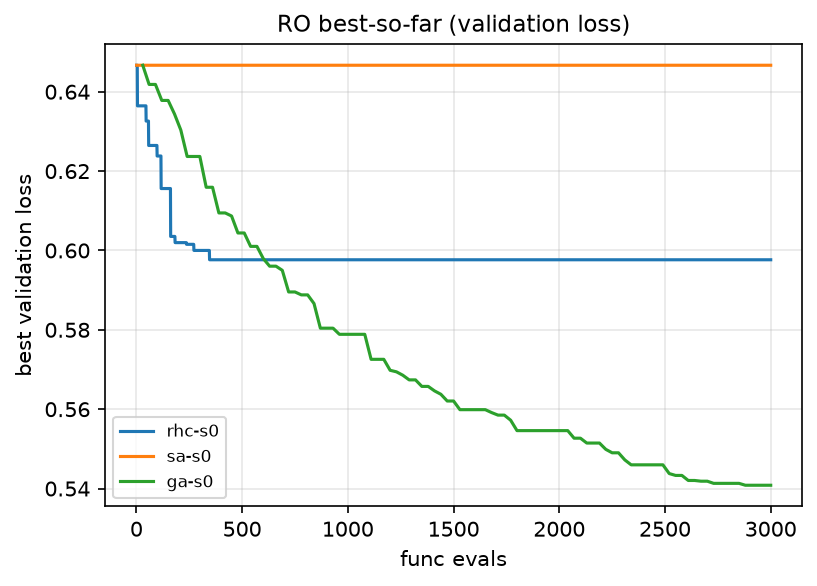
\includegraphics[width=0.92\columnwidth]{outputs/figures/part1_best_so_far}
  \caption{Part~1 RO best-so-far validation loss vs.\ function evaluations
    (seed~0). GA keeps improving (to $0.54$); RHC gains quickly then plateaus at
    $0.60$; SA stays at its $0.65$ initialization. Lower validation loss did
    \emph{not} translate into higher Macro-F1 (Table~\ref{tab:ro}).}
  \label{fig:ro}
\end{figure}

\begin{table}[t]
\caption{Part~1 RO on the final layer ($1{,}057$ params, $3{,}000$ func.\ evals,
  mean over 3 seeds). Best validation loss vs.\ test metrics; SGD baseline shown
  for reference. Lower loss (GA) $\ne$ higher Macro-F1.}
\label{tab:ro}
\centering\small
\begin{tabular}{@{}lrrrrr@{}}
\toprule
Method & Val loss & Acc & Macro-F1 & Bal.Acc & Time\,(s) \\
\midrule
SGD baseline & 0.686 & 0.715 & \textbf{0.625} & 0.767 & 11 \\
RHC          & 0.614 & 0.650 & 0.564 & 0.739 & 43 \\
SA           & 0.665 & 0.700 & 0.612 & 0.764 & 44 \\
GA           & \textbf{0.544} & 0.660 & 0.578 & 0.755 & 43 \\
\bottomrule
\end{tabular}
\end{table}

%-------------------------------------------------------------------------------
\section{Part 2: Adam-Family Optimizer Ablations}
\label{sec:part2}

We train the full backbone with seven optimizers under the fixed $100$-epoch
budget. Learning rates come from a coarse per-family pilot search on
training/validation data only (SGD-family best at $0.1$, matching SL;
Adam-family at $10^{-3}$); AdamW uses decoupled weight decay $10^{-2}$. The
speed-to-target threshold $\ell{=}0.70$ was chosen from the baseline pilot (the
SGD baseline settles near $0.69$), never from test data. ``Adam without bias
correction'' is a custom optimizer that removes the $(1-\beta^t)$ terms; its
update rule is documented in the reproducibility code.

\subsection{Trajectories, threshold, and stability}
Fig.~\ref{fig:part2}(a) plots validation loss versus gradient evaluations and
exposes three regimes. \emph{Adam without bias correction} descends fastest
early---reaching $\ell$ in only $\approx\!533$ gradient evaluations versus
$1{,}233$ for Adam and $1{,}800$ for SGD (Table~\ref{tab:part2}). This is
quantitatively expected: at step $t{=}1$ the uncorrected update is
$(1-\beta_1)/\sqrt{1-\beta_2}=0.1/\sqrt{0.001}\approx3.2\times$ larger than the
bias-corrected one, so no-bias Adam takes larger early steps and crosses the
threshold sooner~\cite{kingma2015}, at the cost of a slightly higher final
validation loss.
\emph{Momentum and Nesterov} diverge upward after $\sim\!4{,}000$ evaluations:
their validation loss climbs to $0.89$ and $0.95$ with the largest
train--validation gaps ($0.64$ and $0.82$), showing that adding momentum at
$\mathrm{lr}{=}0.1$ overshoots and overfits. \emph{Plain SGD} reaches the lowest
\emph{final} validation loss ($0.686$) and is the most seed-stable
(Macro-F1 std $0.001$), but not the best test Macro-F1. The best classification
behavior comes from the RMSProp-like variant ($\beta_1{=}0$): test Macro-F1
$0.649$ and balanced accuracy $0.773$, both the highest in the study
(Fig.~\ref{fig:stab}). That $\beta_1{=}0$ matches or beats full Adam indicates
adaptive second-moment scaling, not first-moment smoothing, drives the gains on
this backbone. AdamW attains the smallest generalization gap among adaptive
methods ($0.331$) via decoupled weight decay, but not the best
Macro-F1---consistent with decoupled decay acting on generalization rather than
optimization speed~\cite{loshchilov2019}.

\begin{figure*}[t]
  \centering
  \subfloat[Validation loss vs.\ gradient evaluations]{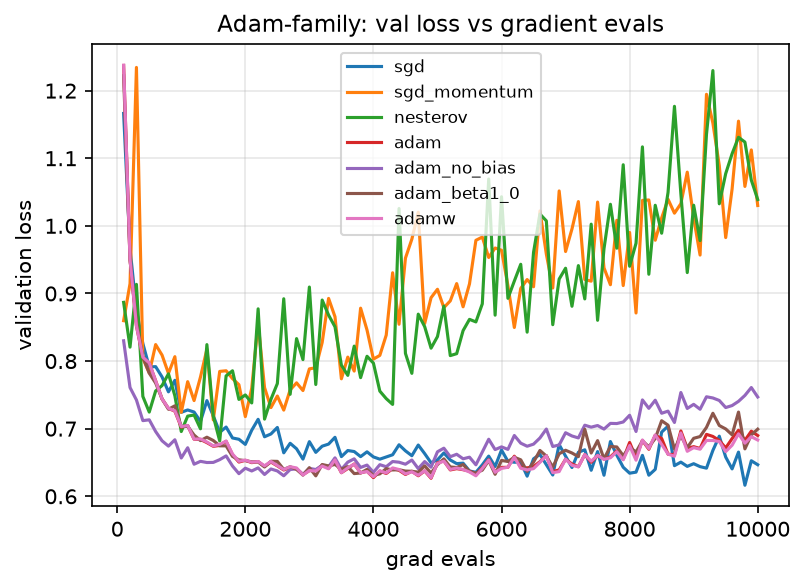
\includegraphics[width=0.9\columnwidth]{outputs/figures/part2_trajectories}}
  \hfill
  \subfloat[Validation loss vs.\ wall-clock time]{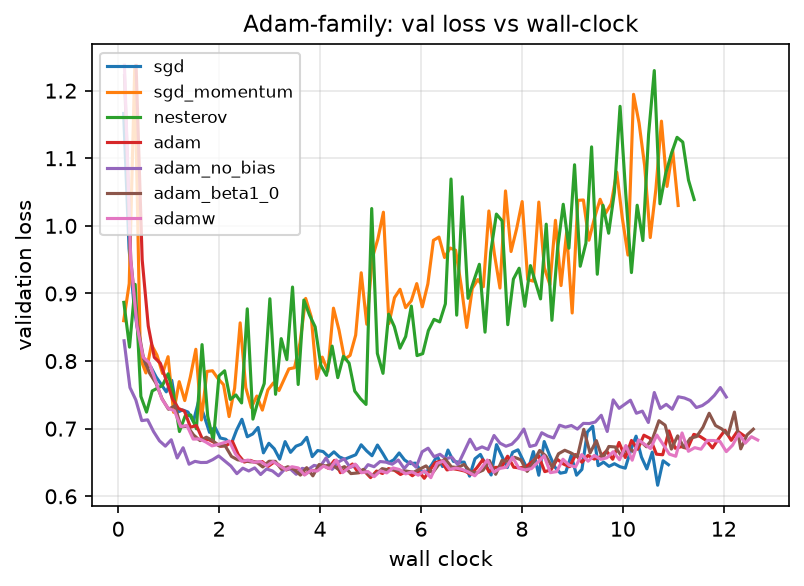
\includegraphics[width=0.9\columnwidth]{outputs/figures/part2_trajectories_time}}
  \caption{Part~2 optimizer trajectories (seed~0), plotted against both compute
    budgets. Momentum and Nesterov diverge/overfit after $\sim\!4$k evaluations
    ($\sim\!6$\,s); Adam-family and SGD stay in the $0.62$--$0.75$ band;
    \emph{adam\_no\_bias} descends fastest early. The two axes agree because all
    seven optimizers share the $10{,}000$-gradient-evaluation budget and similar
    per-step cost ($11$--$13$\,s per run), so wall-clock adds no new ranking here.}
  \label{fig:part2}
\end{figure*}

\begin{figure}[t]
  \centering
  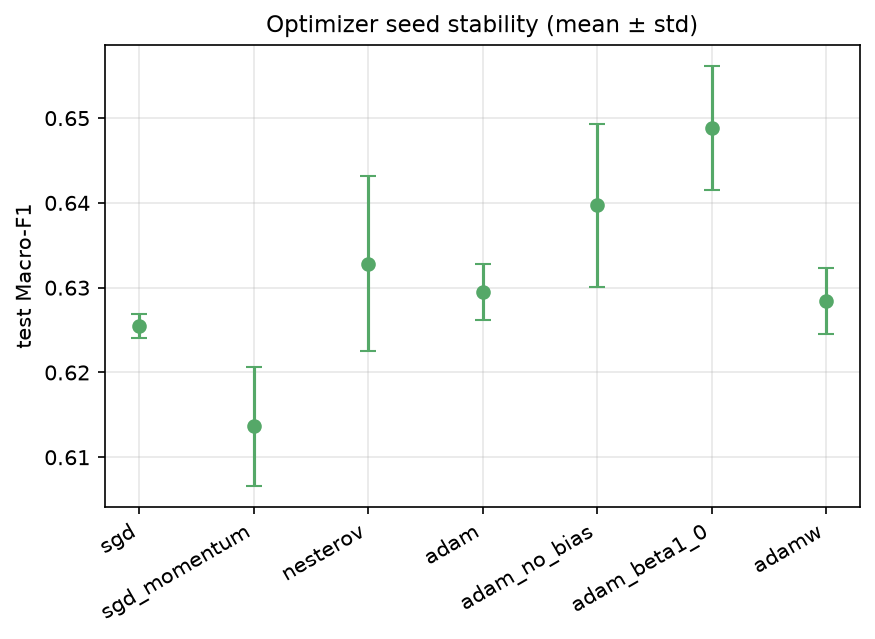
\includegraphics[width=0.88\columnwidth]{outputs/figures/report_part2_stability}
  \caption{Seed stability of test Macro-F1 (three seeds $\{0,1,2\}$, mean $\pm$
    std). The RMSProp-like variant ($\beta_1{=}0$) is highest but with a wide
    band ($\pm0.007$); plain SGD is the tightest ($\pm0.001$) though not the
    strongest. Seed stability and generalization are distinct axes: SGD is the
    most \emph{stable} yet has neither the best test Macro-F1 nor the lowest
    train--validation gap.}
  \label{fig:stab}
\end{figure}

\begin{table}[t]
\caption{Part~2 optimizer ablation (mean over 3 seeds, $10{,}000$ gradient
  evaluations each). Gen.\ gap = final (val $-$ train) loss; $n_\ell$ = gradient
  evaluations to reach $\ell{=}0.70$ (``--'' = not reached by all seeds);
  $\sigma_{F1}$ = seed std of Macro-F1.}
\label{tab:part2}
\centering\scriptsize
\begin{tabular}{@{}lrrrrrrr@{}}
\toprule
Optimizer & lr & Val & Macro & Bal & Gen & $n_\ell$ & $\sigma_{F1}$ \\
          &    & loss & F1 & Acc & gap &          &  \\
\midrule
SGD              & 0.1  & \textbf{0.686} & 0.626 & 0.767 & \textbf{0.259} & 1800 & \textbf{.001} \\
SGD+momentum     & 0.1  & 0.891 & 0.614 & 0.740 & 0.640 & 2100 & .007 \\
Nesterov         & 0.1  & 0.952 & 0.633 & 0.742 & 0.818 & 1550 & .010 \\
Adam             & $10^{-3}$ & 0.814 & 0.629 & 0.766 & 0.356 & 1233 & .003 \\
Adam no-bias     & $10^{-3}$ & 0.856 & 0.640 & 0.766 & 0.433 & \textbf{533} & .010 \\
Adam $\beta_1{=}0$ & $10^{-3}$ & 0.826 & \textbf{0.649} & \textbf{0.773} & 0.354 & 1233 & .007 \\
AdamW            & $10^{-3}$ & 0.790 & 0.628 & 0.767 & 0.331 & 1233 & .004 \\
\bottomrule
\end{tabular}
\end{table}

\subsection{Sensitivity heatmaps}
Fig.~\ref{fig:heat} sweeps coarse $(\alpha,\beta_1)$ and $(\alpha,\beta_2)$ grids
for Adam (short budget). The learning rate $\alpha$ dominates: validation loss is
minimized in a broad, forgiving band at $\alpha{=}10^{-3}$ ($0.64$), underfits at
$\alpha{=}3{\times}10^{-4}$ ($0.71$), and rises again at $3{\times}10^{-3}$
($0.68$). Both $\beta_1$ and $\beta_2$ have weak effects: across each column the
loss varies by $\le0.01$, with only a mild penalty for the shortest
second-moment memory ($\beta_2{=}0.99$) at the largest step size. The near-flat
$\beta_1$ axis corroborates the ablation finding that removing first-moment
smoothing ($\beta_1{=}0$) costs little, so adaptive scaling---not
momentum---carries Adam's benefit here.

\begin{figure*}[t]
  \centering
  \subfloat[$(\alpha,\beta_1)$ sensitivity]{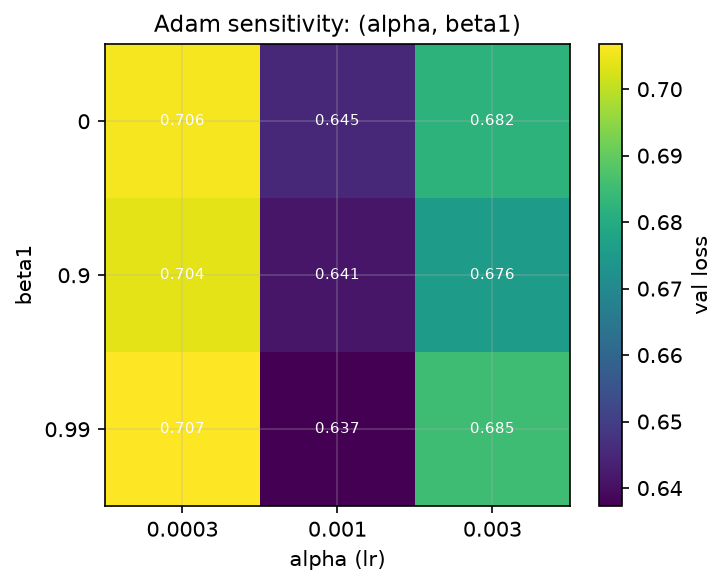
\includegraphics[width=0.78\columnwidth]{outputs/figures/part2_heatmap_beta1}}
  \hfill
  \subfloat[$(\alpha,\beta_2)$ sensitivity]{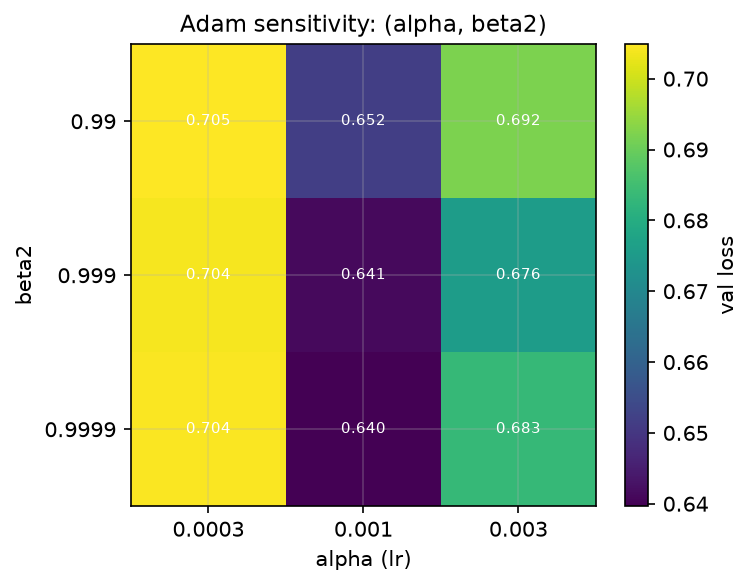
\includegraphics[width=0.78\columnwidth]{outputs/figures/part2_heatmap_beta2}}
  \caption{Adam coarse sensitivity (validation loss). The learning rate is the
    dominant axis with a broad optimum at $\alpha{=}10^{-3}$; both $\beta$ axes
    are nearly flat ($\le0.01$ variation), indicating Adam is forgiving in its
    momentum/second-moment coefficients but sensitive to step size.}
  \label{fig:heat}
\end{figure*}

%-------------------------------------------------------------------------------
\section{Part 3: Regularization Study}
\label{sec:part3}

We fix standard Adam ($\mathrm{lr}{=}10^{-3}$, $\beta{=}(0.9,0.999)$, the best
Part~2 setting) and vary only regularization: coupled L2 weight decay
($\{10^{-5},10^{-4},10^{-3}\}$), early stopping (patience $8$ on validation loss,
restore best), dropout ($\{0.1,0.3,0.5\}$ on the hidden layer), label smoothing
($\{0.05,0.1\}$), and train-only Gaussian input noise
($\sigma\in\{0.05,0.1\}$ in scaled space). Selection uses mean validation loss
across seeds only; the test set is final-only. The best single regularizer and a
data-driven best combination (best member of each family that beats the Adam
baseline) are reported in Table~\ref{tab:part3} and Fig.~\ref{fig:reg}.

\subsection{Interpretation}
Regularization behaves exactly as H2 predicts: it moves the generalization gap
and class balance far more than it moves Macro-F1. \textbf{L2 ($10^{-3}$)} is the
strongest single technique by validation loss ($0.620$ vs.\ the Adam baseline's
$0.697$): it \emph{halves} the train--validation gap ($0.163$ vs.\ $0.356$) and
gives the highest balanced accuracy ($0.774$) and strong minority recall
(C4 recall $0.77$, C5 $0.95$), yet it \emph{lowers} Macro-F1 to $0.600$ because
the extra minority recall costs majority precision. The Adam baseline and the
lightest decay ($10^{-5}$) retain the best Macro-F1 ($0.630$, $0.628$),
confirming that on this backbone the un-regularized optimizer already sits near
the Macro-F1 frontier and further regularization trades aggregate F1 for balance
and a smaller gap. \textbf{Label smoothing fails} here: combined with
class-weighted cross-entropy it inflates the loss scale (validation ``loss''
$1.55$ and $2.17$ are not comparable to un-smoothed cross-entropy) and, more
tellingly, collapses test Macro-F1 to $0.50$ and $0.35$, because softened targets
blunt the sharp minority decisions the weighting is trying to create. The
\textbf{data-driven best combination} (L2 $10^{-3}$ + dropout $0.5$ + input noise
$0.1$), selected purely by validation loss, drives the generalization gap to
essentially zero ($0.008$) and raises C4 recall to $0.81$, but \emph{over-regularizes}
for classification: Macro-F1 drops to $0.542$ and every per-class F1 falls
(Fig.~\ref{fig:cm}). This is itself a key result---selecting by validation loss
does not select for Macro-F1---and it explains why the best combination is
smaller and more targeted than ``all regularizers at once.''

\begin{figure}[t]
  \centering
  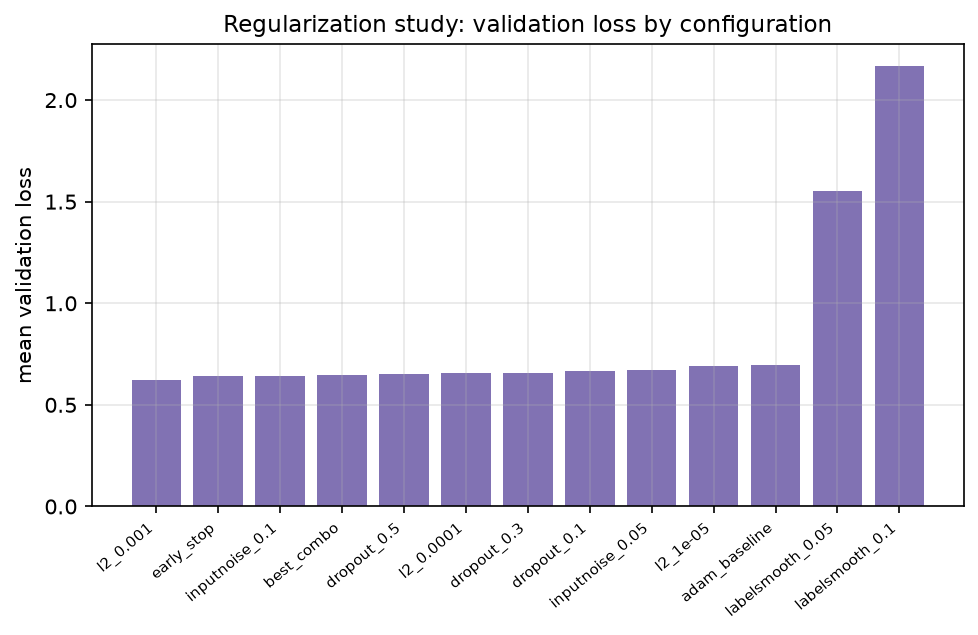
\includegraphics[width=0.98\columnwidth]{outputs/figures/report_part3_regularization}
  \caption{Part~3 mean validation loss by configuration. L2 ($10^{-3}$) is the
    best single regularizer; most techniques cluster near the Adam baseline;
    label smoothing (right) inflates the class-weighted loss and harms
    classification. Selection by validation loss favors heavy regularization
    that lowers Macro-F1 (Table~\ref{tab:part3}).}
  \label{fig:reg}
\end{figure}

\begin{table}[t]
\caption{Part~3 regularization (standard Adam fixed; mean over 3 seeds). Gap =
  train--validation loss gap. Label-smoothing loss is not comparable to
  un-smoothed CE. Best single = L2\,$10^{-3}$; combo = L2$+$dropout$+$noise.}
\label{tab:part3}
\centering\small
\begin{tabular}{@{}lrrrrr@{}}
\toprule
Config & Val loss & Macro-F1 & Bal.Acc & Gap & C4 rec. \\
\midrule
Adam baseline      & 0.697 & \textbf{0.630} & 0.766 & 0.356 & 0.63 \\
L2 $10^{-3}$       & \textbf{0.620} & 0.600 & \textbf{0.774} & 0.163 & 0.77 \\
Dropout $0.5$      & 0.654 & 0.581 & 0.756 & 0.148 & 0.65 \\
Input noise $0.1$  & 0.644 & 0.597 & 0.766 & 0.202 & 0.68 \\
Early stopping     & 0.643 & 0.573 & 0.755 & 0.175 & 0.75 \\
Label smooth $0.1$ & 2.166 & 0.354 & 0.591 & 0.085 & 0.82 \\
Best combination   & 0.649 & 0.542 & 0.755 & \textbf{0.008} & \textbf{0.81} \\
\bottomrule
\end{tabular}
\end{table}

%-------------------------------------------------------------------------------
\section{Part 4: Integrated Best Combination (Extra Credit)}
\label{sec:part4}

We compose the best pieces without new search: standard Adam ($10^{-3}$), the
best Part~3 combination, and the best Part~1 RO method (GA, selected by mean best
validation loss) fine-tuning the same final layer under $10\%$ of the Part~1
budget ($300$ function evaluations). Across three seeds, GA fine-tuning did
\emph{not} improve the recipe: mean Macro-F1 moved from $0.555$ to $0.544$ and
balanced accuracy from $0.760$ to $0.755$, while validation loss fell slightly
($\approx\!0.62$). The direction is exactly the Part~1 dissociation in miniature:
the last-layer search lowers weighted cross-entropy but nudges predictions away
from the minority balance the recipe was chosen for. The integrated recipe also
sits below the best single-part results (the RMSProp-like optimizer's $0.649$),
because it inherits the over-regularized combination's low Macro-F1. We conclude
the extra compute is not justified.

\begin{table}[t]
\caption{Final summary and compute accounting: SL baseline vs.\ the best of each
  part (mean over 3 seeds). Grad = gradient evaluations, Func = RO function
  evaluations. RO/integrated grad counts include the backbone training that
  precedes the last-layer search.}
\label{tab:final}
\centering\scriptsize
\begin{tabular}{@{}lrrrrrr@{}}
\toprule
Method & Val & Macro & Bal & Grad & Func & Time \\
       & loss & F1 & Acc & evals & evals & (s) \\
\midrule
SL SGD baseline            & 0.686 & 0.625 & 0.767 & 10k & 0    & 11 \\
Best opt (Adam $\beta_1{=}0$) & 0.826 & \textbf{0.649} & \textbf{0.773} & 10k & 0 & 13 \\
Best reg (L2 $10^{-3}$)    & \textbf{0.620} & 0.600 & \textbf{0.774} & 10k & 0 & 12 \\
Best RO (GA, final layer)  & 0.544 & 0.578 & 0.755 & 10k & 3k & 54 \\
Integrated (Part 4)        & 0.622 & 0.544 & 0.755 & 10k & 0.3k & 52 \\
\bottomrule
\end{tabular}
\end{table}

\begin{figure}[t]
  \centering
  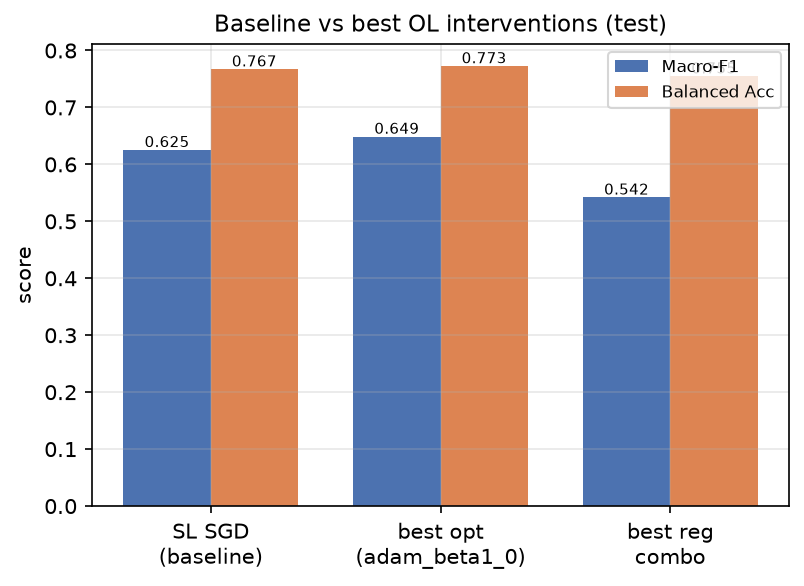
\includegraphics[width=0.92\columnwidth]{outputs/figures/report_baseline_comparison}
  \caption{SL SGD baseline vs.\ the best OL interventions (test, mean over 3
    seeds). The RMSProp-like optimizer ($\beta_1{=}0$) is the only intervention
    that improves on the baseline for both Macro-F1 ($0.649$ vs.\ $0.625$) and
    balanced accuracy ($0.773$ vs.\ $0.767$); the validation-loss-selected
    regularization combination raises balanced accuracy little and \emph{lowers}
    Macro-F1, the over-regularization effect discussed in Section~\ref{sec:part3}.}
  \label{fig:basecmp}
\end{figure}

%-------------------------------------------------------------------------------
\section{Discussion}
\label{sec:discussion}

\subsection{Cross-part synthesis}
Fig.~\ref{fig:basecmp} and Table~\ref{tab:final} summarize the headline
comparison. The three parts tell one coherent story once optimization, generalization,
stability, and efficiency are kept distinct. \emph{Optimization speed} is won by
adaptive scaling: Adam without bias correction reaches the $\ell{=}0.70$
threshold in a third of SGD's gradient evaluations, and the sensitivity sweep
shows a broad, forgiving learning-rate optimum. \emph{Generalization} is a
different axis: plain SGD reaches the lowest final validation loss and the RMSProp-like
Adam variant the best Macro-F1/balanced accuracy, while momentum and Nesterov,
though fast, overfit the most (gaps $0.64$--$0.82$); among adaptive methods,
AdamW's decoupled weight decay and L2 in Part~3 are what actually shrink the
train--validation gap. \emph{Stability} favors SGD (Macro-F1 std $0.001$) over the
higher-variance adaptive variants, so the RMSProp-like optimizer's Macro-F1 edge
comes with a wider seed band and should be claimed cautiously---seed stability and
generalization are separate axes here. \emph{Efficiency} condemns final-layer RO:
it spent $\sim\!4\times$ the wall-clock of a full training run to \emph{reduce}
Macro-F1. Fig.~\ref{fig:pareto} places every method on a Macro-F1-versus-compute
frontier and makes this concrete: all three RO variants sit far to the right
(more compute) and below the baseline line, while the RMSProp-like optimizer is
the top-left (best metric, least compute) point. The recurring theme is a
\emph{loss--F1 dissociation}: GA (Part~1), heavy regularization (Part~3), and the
integrated recipe (Part~4) all lowered validation loss while lowering Macro-F1,
because class-weighted cross-entropy rewards majority-class \emph{confidence}
whereas Macro-F1 rewards the minority-class \emph{decision boundary}---the two
objectives are only loosely coupled, so ``lowest loss'' need not mean ``best F1.''

\begin{figure}[t]
  \centering
  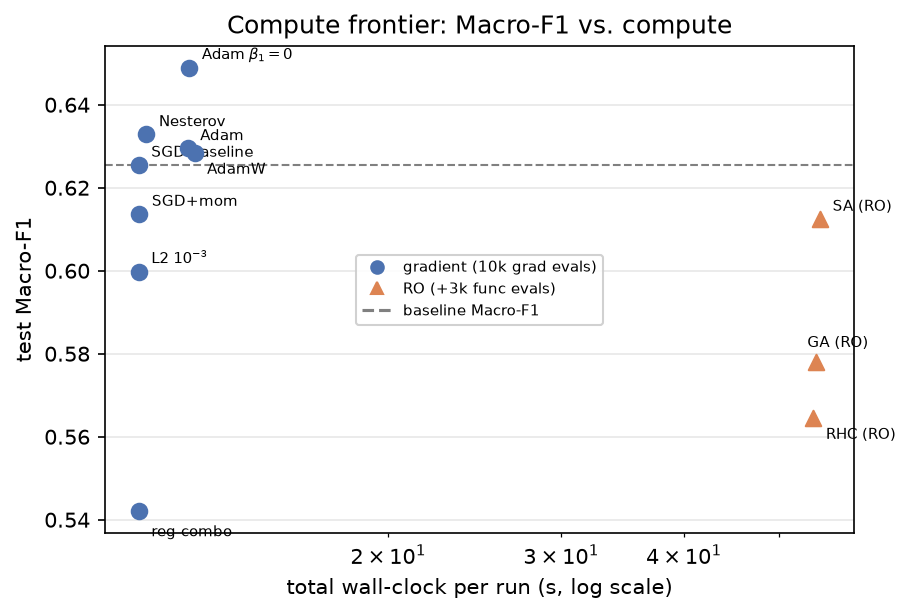
\includegraphics[width=0.94\columnwidth]{outputs/figures/report_pareto_compute}
  \caption{Compute frontier: test Macro-F1 vs.\ total wall-clock per run
    (log scale). Gradient methods (circles) cost $11$--$13$\,s; RO (triangles)
    adds $3{,}000$ function evaluations ($\sim\!43$\,s) on top of backbone
    training. Every RO variant lies below the baseline (dashed) at $\sim\!4\times$
    the compute; the RMSProp-like optimizer dominates the frontier. This is the
    visual case for ``final-layer RO is not worth the compute.''}
  \label{fig:pareto}
\end{figure}

\subsection{Class-level behavior}
The confusion matrices (Fig.~\ref{fig:cm}) show that all models share the
mid-elevation C1$\leftrightarrow$C2 confusion inherited from the SL analysis
(e.g.\ $403$ C2 instances predicted as C1 in the baseline). Class weighting keeps
minority classes visible---the baseline recovers $15/19$ C4 instances---and the
strongly regularized combination raises C4 recall further to $0.81$, but by
pushing majority instances into minority buckets (e.g.\ $311$ C2\,$\to$\,C5),
which lowers minority \emph{precision} and every per-class F1. A method that
improves minority recall is therefore not simply ``better''; the balanced-accuracy
gain from L2 is real, but its Macro-F1 cost is equally real. The per-class view
(Fig.~\ref{fig:pcf1}) sharpens this: the minority classes C4 (Cottonwood, $19$
test instances) and especially C5 (Aspen) hold the lowest F1 and drive the
Macro-F1 gap; the RMSProp-like optimizer improves \emph{every} class over the
baseline (C5 $0.40$ vs.\ $0.37$, C7 $0.72$ vs.\ $0.67$), whereas the regularized
combination is uniformly worse, confirming it over-regularizes rather than
rebalancing.

\begin{figure}[t]
  \centering
  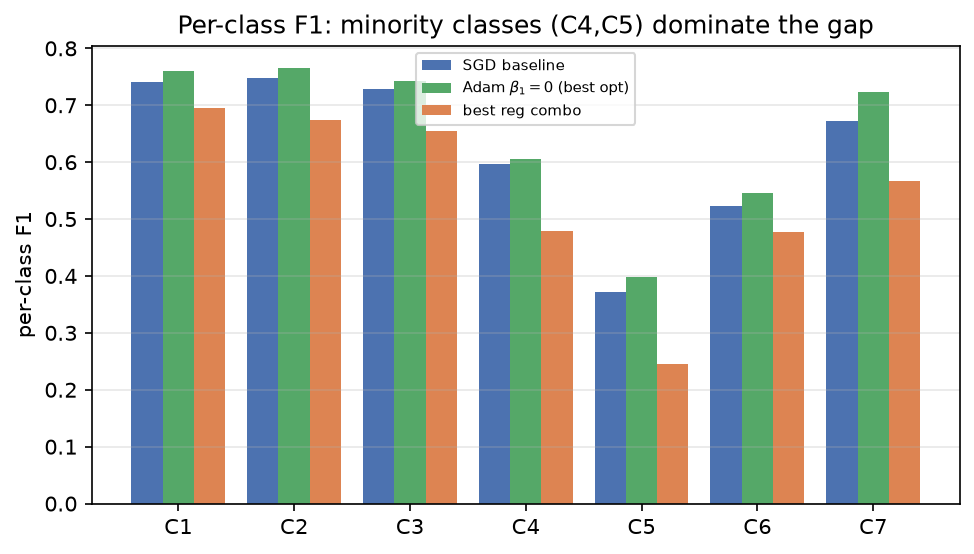
\includegraphics[width=0.98\columnwidth]{outputs/figures/report_perclass_f1}
  \caption{Per-class test F1 (mean over 3 seeds). Minority classes C4/C5 hold the
    lowest F1 and dominate the Macro-F1 gap. The RMSProp-like optimizer
    ($\beta_1{=}0$) improves every class over the SL baseline; the
    validation-loss-selected regularization combination is uniformly worse.}
  \label{fig:pcf1}
\end{figure}

\begin{figure*}[t]
  \centering
  \subfloat[SL SGD baseline]{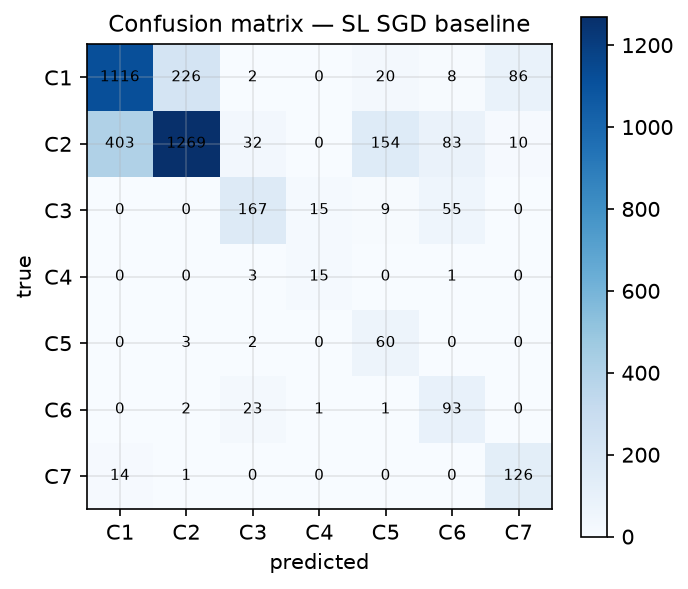
\includegraphics[width=0.80\columnwidth]{outputs/figures/report_confusion_baseline}}
  \hfill
  \subfloat[Best regularized Adam combination]{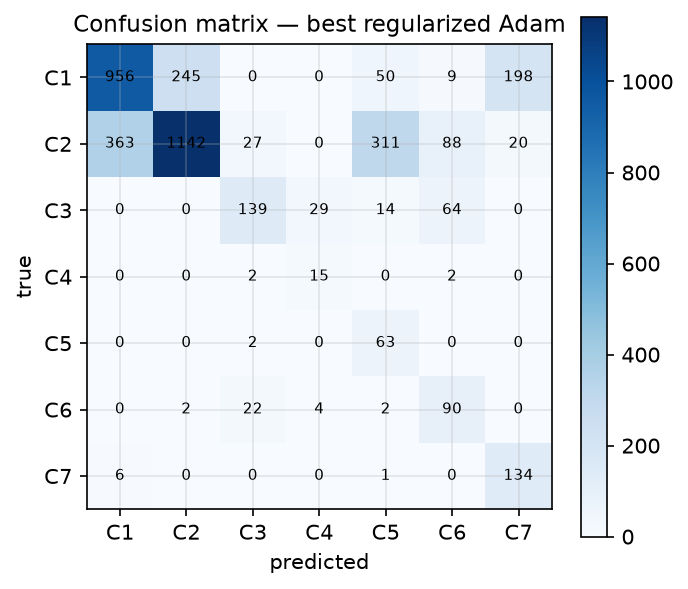
\includegraphics[width=0.80\columnwidth]{outputs/figures/report_confusion_best}}
  \caption{Class-level behavior (test, seed~0). Both share the
    C1$\leftrightarrow$C2 confusion. The regularized combination raises minority
    recall (C4 $15/19$; more mass into C5) but spreads majority mass into
    minority columns, lowering precision and per-class F1---why its Macro-F1 is
    lower despite a near-zero generalization gap.}
  \label{fig:cm}
\end{figure*}

\subsection{Limitations}
Conclusions are specific to this study. The $20{,}000$-instance sample leaves C4
with $19$ test instances, so its per-class F1 carries $\approx\!\pm0.2$
uncertainty and the minority-recall gains are noisy. RO is confined to the
$1{,}057$-parameter final layer under a $3{,}000$-evaluation budget, so a negative
RO result does not generalize to whole-network search. Adam heatmaps are coarse
($3{\times}3$) and use a shortened budget, so weak $\beta$ effects may partly
reflect the short horizon. Only three seeds support the stability claims, and all
conclusions are conditioned on this fixed single-hidden-layer backbone and the
class-weighted loss; a wider or deeper network, or an unweighted loss, could
shift the optimizer/regularizer trade-offs.

\subsection{Decision rule and hypothesis resolution}
\textbf{Decision rule for Covertype (ordered).} \emph{(1)} Fix the learning rate
first---it dominates Adam behavior (Fig.~\ref{fig:heat}); use $\alpha\!\approx\!10^{-3}$.
\emph{(2)} For the best test Macro-F1/balanced accuracy, choose the RMSProp-like
Adam variant ($\beta_1{=}0$); remove bias correction only if early
speed-to-threshold matters, not for final quality. \emph{(3)} If the
train--validation gap or minority recall is the concern, add \emph{one} modest
regularizer---L2 at $10^{-3}$ (or AdamW's decoupled decay)---rather than stacking
several, which over-regularizes and depresses Macro-F1; avoid label smoothing
under class-weighted loss. \emph{(4)} Do not spend compute on final-layer RO for
performance: use it only as a diagnostic, since its validation-loss gains did not
transfer to Macro-F1 at $\sim\!4\times$ the compute. This ordering may not
transfer to datasets with different imbalance, feature scaling, or sample size.
\textbf{Resolution.} \emph{H1 is accepted}: adaptive scaling reached $\ell$
fastest (no-bias Adam in $533$ vs.\ SGD's $1{,}800$ gradient evaluations), yet the
fastest and lowest-loss methods were not the best on Macro-F1. \emph{H2 is
accepted}: L2 halved the generalization gap and moved balanced accuracy and C4
recall more than any optimizer swap, while barely helping (often hurting)
Macro-F1. \emph{H3 is accepted}: final-layer RO produced lower validation loss but
equal-or-worse Macro-F1 at $\sim\!4\times$ the compute, in Part~1 and again in the
Part~4 integration.

%-------------------------------------------------------------------------------
\section*{AI Use Statement}
I used Claude (Anthropic) to brainstorm and outline sections, generate and
refactor small Python code snippets and plotting utilities, debug the experiment
harness, and edit grammar and clarity. All experimental design, hypotheses,
analysis, and interpretations are my own, and I reviewed, verified, and
understood all assisted content and results.

%-------------------------------------------------------------------------------
\begin{thebibliography}{99}
\small

\bibitem{blackard1999}
J.\,A.\ Blackard and D.\,J.\ Dean, ``Comparative accuracies of artificial neural
networks and discriminant analysis in predicting forest cover types from
cartographic variables,'' \textit{Computers and Electronics in Agriculture},
vol.\,24, no.\,3, pp.\,131--151, 1999.

\bibitem{kingma2015}
D.\,P.\ Kingma and J.\ Ba, ``Adam: A method for stochastic optimization,'' in
\textit{Proc.\ Int.\ Conf.\ Learning Representations (ICLR)}, 2015.

\bibitem{loshchilov2019}
I.\ Loshchilov and F.\ Hutter, ``Decoupled weight decay regularization,'' in
\textit{Proc.\ Int.\ Conf.\ Learning Representations (ICLR)}, 2019.

\bibitem{srivastava2014}
N.\ Srivastava, G.\ Hinton, A.\ Krizhevsky, I.\ Sutskever, and R.\ Salakhutdinov,
``Dropout: A simple way to prevent neural networks from overfitting,''
\textit{Journal of Machine Learning Research}, vol.\,15, no.\,1, pp.\,1929--1958,
2014.

\bibitem{muller2019}
R.\ M\"uller, S.\ Kornblith, and G.\ Hinton, ``When does label smoothing help?''
in \textit{Advances in Neural Information Processing Systems (NeurIPS)}, vol.\,32,
2019.

\bibitem{sokolova2009}
M.\ Sokolova and G.\ Lapalme, ``A systematic analysis of performance measures for
classification tasks,'' \textit{Information Processing \& Management}, vol.\,45,
no.\,4, pp.\,427--437, 2009.

\bibitem{he2009}
H.\ He and E.\,A.\ Garcia, ``Learning from imbalanced data,'' \textit{IEEE Trans.\
Knowledge and Data Engineering}, vol.\,21, no.\,9, pp.\,1263--1284, 2009.

\end{thebibliography}

\end{document}
